\begin{tcolorbox}[colback=red!3!white,colframe=red!50!black,boxrule=0.8pt,title={Correction notes},fonttitle=\bfseries]
\textbf{Note on the calculation review (29~Sept.~2026).} The numerical value $c = 299\,792\,458$~m/s has been fixed by definition since 1983 (17th CGPM). Einstein postulated the constancy of $c$ but did not set a numerical value; the document itself states this correctly later on. The rest of the text is unchanged.

\medskip\noindent\textbf{Note on the corpus status: variable speed of light.} The idea of a varying speed of light referred to in this document has been replaced in the later corpus by \emph{fractal path lengthening}: the geometric stretching of the propagation path in the $\xi$ field (Doc.~026, 149, 182; achromatic according to K6 in Doc.~190). Statements that rely on a variable speed of light are to be read accordingly.
\end{tcolorbox}

\section*{Abstract}
		This work shows the central point of Einstein's relativity theory: E=mc² is mathematically identical to E=m. The only difference lies in Einstein's treatment of c as a ``constant'' instead of a dynamic ratio. By fixing c = 299,792,458 m/s, the natural time-mass duality T·m = 1 is ``frozen,'' leading to apparent complexity. The T0 theory puts forward the thesis: c is not a fundamental law of nature, but a ratio that must be variable if time is variable. The choice of convention concerned not E=mc² itself, but the constant-setting of c.

	\medskip\noindent\textbf{Note on versions.} The German version of this document is more extensive than this English one. Earlier revisions shortened or changed parts of the English version. Where the two differ, the more extensive German version applies.

	\medskip\noindent\textbf{Status markers.} Statements marked \textbf{[S]} are \emph{speculative}: a hint or conjecture that has not yet been derived or numerically checked in the corpus.

	
	
	
	\section{The Central Thesis: E=mc² = E=m}
	
	\begin{tcolorbox}[colback=red!5!white,colframe=red!75!black,title=The Central Thesis]
		\textbf{E=mc² and E=m are mathematically identical in natural units.}
		
		In the T0 reading, the difference is that Einstein treats c as a ``constant,'' while T0 theory regards c as a dynamic ratio.
		
		\textbf{Einstein's choice}: c = 299,792,458 m/s = constant
		
		\textbf{T0 view}: c = L/T = variable ratio
	\end{tcolorbox}
	
	\subsection{The Mathematical Identity}
	
	\textbf{In natural units}:
	\begin{equation}
		E = mc^2 = m \times c^2 = m \times 1^2 = m
	\end{equation}
	
	\textbf{This is not an approximation but the same equation in different units.}
	
	\subsection{What is c really?}
	
	\begin{equation}
		c = \frac{\text{Length}}{\text{Time}} = \frac{L}{T}
	\end{equation}
	
	\textbf{In the T0 reading, c is a ratio, not a natural constant.}
	
	\section{The Convention Choice: The Constant-Setting of c}
	
	\subsection{The Act of Constant-Setting}
	
	Einstein set: $c = 299,792,458$ m/s = \textbf{constant}
	
	\textbf{What does this mean?}
	\begin{equation}
		c = \frac{L}{T} = \text{constant} \quad \Rightarrow \quad \frac{L}{T} = \text{fixed}
	\end{equation}
	
	\textbf{Implication}: If L and T can vary, their \textbf{ratio} must remain constant.
	
	\subsection{The Problem of Time Variability}
	
	\textbf{Einstein recognized himself}: Time dilates.
	\begin{equation}
		t' = \gamma t \quad \text{(time is variable)}
	\end{equation}
	
	\textbf{At the same time he set}: 
	\begin{equation}
		c = \frac{L}{T} = \text{constant}
	\end{equation}
	
	\textbf{From the T0 viewpoint this is a tension. Relativity theory resolves it through the joint transformation of length and time; T0 theory resolves it in a different way.}
	
	\subsection{The T0 Resolution}
	
	\textbf{T0 insight}: $\Tfield \cdot m = 1$
	
	This means:
	\begin{itemize}
		\item Time $\Tfield$ \textbf{must} be variable (coupled to mass)
		\item Therefore $c = L/T$ \textbf{cannot} be constant
		\item $c$ is a \textbf{dynamic ratio}, not a constant
	\end{itemize}
	
	\section{Constant-Setting from the T0 Viewpoint}
	
	\subsection{The Mechanism of Constant-Setting}
	
	\textbf{Step 1}: Einstein sets c = constant
	\begin{equation}
		c = 299,792,458 \text{ m/s} = \text{fixed}
	\end{equation}
	
	\textbf{Step 2}: Time becomes ``frozen'' by this
	\begin{equation}
		T = \frac{L}{c} = \frac{L}{\text{constant}} = \text{apparently determined}
	\end{equation}
	
	\textbf{Step 3}: Time dilation becomes ``mysterious effect''
	\begin{equation}
		t' = \gamma t \quad \text{(explained via relativity theory)}
	\end{equation}
	
	\subsection{What Really Happens (T0 View)}
	
	\textbf{T0 view}: Time is variable through $\Tfield \cdot m = 1$
	
	\textbf{Einstein's constant-setting} ``freezes'' this variability
	
	\textbf{Result}: The ``frozen'' dynamics must be captured through additional formalism (Lorentz transformations)
	
	\section{c as Ratio vs. c as Constant}
	
	\subsection{c as Natural Ratio (T0)}
	
	\begin{equation}
		c(x,t) = \frac{L(x,t)}{T(x,t)}
	\end{equation}
	
	\textbf{Properties}:
	\begin{itemize}
		\item $c$ varies with location and time
		\item $c$ follows the time-mass duality
		\item No fixed constants
		\item Natural simplicity: $E = m$
	\end{itemize}
	
	\subsection{c as Fixed Constant (Einstein)}
	
	\begin{equation}
		c = 299,792,458 \text{ m/s} = \text{constant everywhere}
	\end{equation}
	
	\textbf{Problems from the T0 viewpoint}:
	\begin{itemize}
		\item Tension with time dilation
		\item ``Freezing'' of time dynamics
		\item Additional formalism needed
		\item Unit factor in the formula: $E = mc^2$
	\end{itemize}
	
	\section{The Time Dilation Paradox}
	
	\subsection{The Tension from the T0 Viewpoint}
	
	\textbf{Relativity theory sets simultaneously}:
	\begin{align}
		c &= \text{constant} \\
		t' &= \gamma t \quad \text{(time varies)}
	\end{align}
	
	\textbf{But}:
	\begin{equation}
		c = \frac{L}{T} \quad \text{and} \quad T \text{ varies} \quad \Rightarrow \quad c \text{ cannot be constant}
	\end{equation}
	
	\subsection{The Solution of Relativity Theory}
	
	Relativity theory handles this through:
	\begin{itemize}
		\item Lorentz transformations
		\item Mathematical formalisms
		\item Space-time constructions
		\item \textbf{From the T0 viewpoint it remains open why c in particular is fixed.}
	\end{itemize}
	
	\subsection{The Solution in T0 Theory}
	
	\textbf{In T0 theory}:
	\begin{equation}
		\Tfield \cdot m = 1 \quad \Rightarrow \quad \text{time is naturally variable}
	\end{equation}
	
	\begin{equation}
		c = \frac{L}{T} \quad \Rightarrow \quad \text{c is naturally variable}
	\end{equation}
	
	\textbf{No constant-setting $\rightarrow$ no such tension $\rightarrow$ no additional formalism}
	
	\section{The Mathematical Demonstration}
	
	\subsection{From E=mc² to E=m}
	
	\textbf{Starting equation}: $E = mc^2$
	
	\textbf{c in natural units}: $c = 1$
	
	\textbf{Substitution}:
	\begin{equation}
		E = mc^2 = m \times 1^2 = m
	\end{equation}
	
	\textbf{Result}: $E = m$
	
	\subsection{The Reverse Direction: From E=m to E=mc²}
	
	\textbf{Starting equation}: $E = m$
	
	\textbf{Introducing the constant}: $c = 299,792,458$ m/s
	
	\textbf{Rewriting the equation}:
	\begin{equation}
		E = m = m \times 1 = m \times \frac{c^2}{c^2} = m \times c^2 \times \frac{1}{c^2}
	\end{equation}
	
	\textbf{If one defines $c^2$ as ``conversion factor''}:
	\begin{equation}
		E = mc^2
	\end{equation}
	
	\textbf{This shows}: $E = mc^2$ is $E = m$ with the \textbf{conversion factor} $c^2$.
	
	\section{The Practical Justification of \( E = mc^2 \) in Our Experiential Realm}
	
	\subsection{\( E = mc^2 \) and \( E = m \) – Same Content in Different Unit Systems}
	
	\begin{tcolorbox}[colback=blue!10!white,colframe=blue!75!black,title=The Pragmatic Perspective: Unit Systems and Conventions]
		The key point: The equation \( E = mc^2 \) is mathematically equivalent to \( E = m \) when one chooses suitable units.
		
		\textbf{Einstein formulated in SI units (practical for our world):}
		\begin{equation}
			E = m \cdot (299\,792\,458)^2 \ \text{J} 
		\end{equation}
		
		\textbf{T0 formulates in natural units (fundamentally simpler):}
		\begin{equation}
			E = m \quad \text{with} \quad c = 1
		\end{equation}
		
		Both descriptions contain exactly the same physical information – they merely use different measuring rods.
		
		The choice between them is not a question of ``right'' or ``wrong,'' but of \textit{practical suitability versus fundamental simplicity}.
	\end{tcolorbox}
	
	\subsection{Why the Fixation \( c = \text{const.} \) Is Practically Reasonable}
	
	\textbf{For our everyday experiential world}, the establishment of \( c \) as a constant is not only historically understandable but also \textit{pragmatically justified} from multiple perspectives:
	
	\begin{enumerate}[leftmargin=*, label=\textbf{\arabic*.}]
		\item \textbf{Measurement Practice:} All our measuring instruments (clocks, rulers, electronic devices) utilize physical processes that themselves depend on \( c \). Establishing a fixed \( c \) creates a consistent reference framework for reproducible experiments. Without such a convention, every measurement would require a circular self-calibration.
		
		\item \textbf{Technological Applications:} From GPS navigation to particle accelerator technology, practical applications are based on the assumption of a locally constant \( c \). This assumption works with extremely high precision for the range in which we live and work. The error introduced by this assumption is far below the resolution of our current technology for most applications.
		
		\item \textbf{Scientific Communication:} A uniform convention allows scientists worldwide to compare results and communicate with each other. The SI units with fixed \( c \) provide a practical basis for this. Science requires shared languages, and measurement conventions form an essential part of this language.
		
		\item \textbf{Historical Development:} The establishment of \( c \) as constant did not occur arbitrarily but emerged from centuries of measurement attempts (Roemer, Fizeau, Michelson-Morley) that within their accuracy showed no variation. Einstein built on this empirical foundation.
		
		\item \textbf{Educational Transmission:} Complex theories require entry points. \( E = mc^2 \) with constant \( c \) provides such an entry point into relativistic thinking. The deeper insight \( E = m \) can follow as a second step for those seeking the fundamental structure.
	\end{enumerate}
	
	\subsection{The Crucial Distinction: Practical Convention vs. Fundamental Natural Law}
	
	\textbf{T0 Theory distinguishes two levels:}
	
	\begin{table}[H]
		\centering
		\adjustbox{max width=\textwidth}{%
\begin{tabular}{|p{6cm}|p{6cm}|}
			\hline
			\textbf{Practical Measurement Convention} & \textbf{Fundamental Natural Law} \\
			\hline
			For technical applications and everyday experiments, fixing \( c = 299\,792\,458 \ \text{m/s} \) is sensible and useful. & On the most fundamental level, \( c \) is not an absolute natural constant but a dynamic ratio \( L/T \) that follows the time-mass duality \( T \cdot m = 1 \). \\
			\hline
			Corresponds to selecting a stable reference system for our world of experience. & Is meant to correspond to the intrinsic structure of reality before any human conventions. \\
			\hline
			Necessary for building reproducible technology and conducting comparable experiments. & Necessary for understanding the ultimate principles behind the phenomena. \\
			\hline
			Works for 99.9\% of all current applications. & Shows what remains when all practical conventions are removed. \\
			\hline
		\end{tabular}%
}
		\caption{The dual nature of physical descriptions}
	\end{table}
	
	\subsection{Einstein's Historical Achievement in New Light}
	
	\begin{tcolorbox}[colback=green!10!white,colframe=green!75!black,title=Einstein's Achievement from the T0 Viewpoint]
		Einstein found the energy-mass equivalence (in natural units \( E = m \)) and formulated it in the \textit{units practical for his time} as \( E = mc^2 \).
		
		\textbf{His historical achievement from the T0 perspective consists of three levels:}
		
		\begin{enumerate}
			\item \textbf{Discovery of the fundamental relationship:} Recognizing that energy and mass are different manifestations of the same reality.
			
			\item \textbf{Pragmatic formulation:} Expressing this insight in a form usable for experiments and verifiable by contemporary measurements.
			
			\item \textbf{Conceptual reorganization:} Drawing the consequences for our space-time conception and thereby overcoming Newtonian absolutism.
		\end{enumerate}
		
		The T0 Theory does not diminish this achievement but shows that behind the practical form \( E = mc^2 \) lies an even more fundamental simplicity \( E = m \). From the T0 viewpoint Einstein stopped one step before this simpler form – a step that was appropriate for his time.
		
		\textbf{Remark:} In natural units Einstein's relation reads \( E = m \); he wrote it as \( E = mc^2 \) because this corresponded to the measurement practices of his time. That both forms express the same statement is familiar in theoretical physics; T0 theory attributes fundamental significance to the simple form.
	\end{tcolorbox}
	
	\subsection{From Practical to Fundamental Description: A Historical Progression}
	
	\textbf{The development of physics} can be understood as a continuous refinement of our reference systems and recognition of which elements are conventions and which are intrinsic structures:
	
	\begin{table}[H]
		\centering
		\resizebox{\textwidth}{!}{%
			\begin{tabular}{|p{3cm}|p{5cm}|p{5cm}|p{5cm}|}
				\hline
				\textbf{Stage} & \textbf{Practical Form} & \textbf{Fundamental Insight} & \textbf{Historical Context} \\
				\hline
				Newtonian Physics & \( F = m \cdot a \) (with absolute time and space) & Approximation for \( v \ll c \) & Industrial Age: Machines, mechanics, predictable motion \\
				\hline
				Einstein (Special Relativity) & \( E = mc^2 \) (with \( c = \text{const.} \)) & Energy-mass equivalence & Early 20th Century: Electromagnetism, early atomic physics \\
				\hline
				Einstein (General Relativity) & \( G_{\mu\nu} = \frac{8\pi G}{c^4} T_{\mu\nu} \) (10 field equations) & Geometry as gravity & Age of astronomy, cosmology \\
				\hline
				Quantum Mechanics & \( i\hbar \frac{\partial}{\partial t} \psi = H \psi \) & Quantization of energy & Atomic and nuclear age \\
				\hline
				T0 Theory & \( E = m \) in natural units (with \( T \cdot m = 1 \)) & Time-mass duality as fundamental & Information Age: Search for unified principles \\
				\hline
		\end{tabular}}
		\caption{Historical progression from practical to fundamental descriptions}
	\end{table}
	
	\textbf{Each stage} retains the validity of the previous ones for their application area but expands understanding to a deeper level. Newton is not ``wrong'' but limited in scope. Einstein is not ``wrong'' but stopped at a certain level of convention. T0 seeks to go one step further – but does not invalidate the previous steps.
	
	\subsection{Coexistence of Both Descriptions: A Peaceful Expansion}
	
	\textbf{T0 Theory proposes not a break with established physics but a peaceful expansion:}
	
	\begin{itemize}
		\item \textbf{For 99.9\% of all technical applications:} \( E = mc^2 \) with constant \( c \) remains the practical and correct formulation. All engineering, GPS technology, particle accelerators, and space travel can continue to work with the established equations.
		
		\item \textbf{For fundamental theoretical questions:} \( E = m \) in natural units shows the actual simplicity of the energy-mass relationship and avoids the tension described above (the time dilation paradox from the T0 viewpoint). Theoretical physicists gain a simpler, more consistent foundation.
		
		\item \textbf{For future precision experiments:} The possibility of tiny \( c \) variations (as predicted by T0) should be kept in mind. Experiments can be designed to test whether \( c \) is \textit{exactly} constant or only \textit{practically} constant within our measurement accuracy.
		
		\item \textbf{For educational purposes:} The relationship can be taught at two levels: first the practical level \( E = mc^2 \) (as done today), then the fundamental level \( E = m \) for advanced students. This corresponds to teaching Newtonian mechanics before relativity.
	\end{itemize}
	
	\begin{tcolorbox}[colback=yellow!10!white,colframe=yellow!75!black,title=The Peaceful Expansion]
		The insight that \( E = mc^2 = E = m \) does not require us to discard existing physics books or redesign technical systems. It only requires us to recognize that we have been working with a particularly practical form of a simpler basic form.
		
		\textbf{The change is conceptual, not practical.}
	\end{tcolorbox}
	
	\subsection{The Actual Concern of T0 Theory}
	
	\begin{tcolorbox}[colback=orange!10!white,colframe=orange!75!black,title=The Concern of T0 Theory]
		T0 does not want to abolish \( E = mc^2 \) as a practical equation but to show:
		
		\textbf{That behind the practical form lies a fundamental simplicity that has been obscured by the historical choice of units.}
		
		This insight does not free us from the necessity of practical conventions but opens a deeper understanding of what these conventions actually describe.
		
		\textbf{The goal:} Not to make physics more complicated, but to recognize its inherent simplicity – and then consciously choose which level of description is appropriate for which purpose.
	\end{tcolorbox}
	
	\subsection{The Double Perspective: Practical Engineering vs. Fundamental Science}
	
	\textbf{The T0 view allows a double perspective:}
	
	\begin{figure}[H]
		\centering
		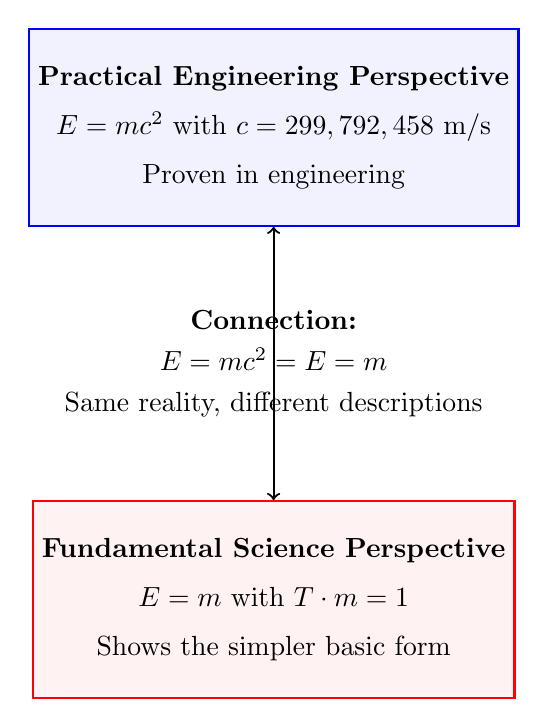
\begin{tikzpicture}[node distance=1.5cm]
			\node (practical) [rectangle, draw=blue, thick, fill=blue!5, minimum width=6cm, minimum height=2.5cm, align=center] {\textbf{Practical Engineering Perspective}\\[0.2cm]$E = mc^2$ with $c = 299,792,458$ m/s\\[0.2cm]Proven in engineering};
			
			\node (fundamental) [rectangle, draw=red, thick, fill=red!5, minimum width=6cm, minimum height=2.5cm, align=center, below of=practical, yshift=-4.5cm] {\textbf{Fundamental Science Perspective}\\[0.2cm]$E = m$ with $T \cdot m = 1$\\[0.2cm]Shows the simpler basic form};
			
			\draw[<->, thick] (practical.south) -- (fundamental.north);
			\node at (0,-3) [align=center] {\textbf{Connection:}\\[0.1cm]$E = mc^2 = E = m$\\[0.1cm]Same reality, different descriptions};
		\end{tikzpicture}
		\caption{The double perspective of T0 Theory}
	\end{figure}
	
	\textbf{Both perspectives are valid and useful – for different purposes.} The engineer needs the practical perspective to build reliable technology. The theoretical physicist seeks the fundamental perspective to understand ultimate principles. T0 shows that these are not contradictory but complementary views of the same reality.
	
	\section{The Arbitrariness of Constant Choice: c or Time?}
	
	\subsection{Einstein's Choice}
	
	\begin{tcolorbox}[colback=orange!5!white,colframe=orange!75!black,title=The Fundamental Choice Option]
		\textbf{One can choose what should be ``constant''.}
		
		\textbf{Option 1 (Einstein's choice)}: c = constant $\rightarrow$ time becomes variable
		
		\textbf{Option 2 (alternative)}: time = constant $\rightarrow$ c becomes variable
		
		\textbf{Both describe the same physics.}
	\end{tcolorbox}
	
	\subsection{Option 1: Einstein's c-constant}
	
	\textbf{Einstein chose}:
	\begin{align}
		c &= 299,792,458 \text{ m/s} = \text{constant (defined)} \\
		t' &= \gamma t \quad \text{(time becomes automatically variable)}
	\end{align}
	
	\textbf{Language convention}:
	\begin{itemize}
		\item ``Speed of light is universally constant''
		\item ``Time dilates in strong gravitational fields''
		\item ``Clocks run slower at high velocities''
	\end{itemize}
	
	\subsection{Option 2: Time-constant (Einstein could have chosen)}
	
	\textbf{Alternative choice}:
	\begin{align}
		t &= \text{constant (defined)} \\
		c(x,t) &= \frac{L(x,t)}{t} = \text{variable}
	\end{align}
	
	\textbf{Alternative language convention}:
	\begin{itemize}
		\item ``Time flows equally everywhere''
		\item ``Speed of light varies with location''
		\item ``Light becomes slower in strong gravitational fields''
	\end{itemize}
	
	\subsection{Mathematical Equivalence of Both Options}
	
	\textbf{Both descriptions are mathematically identical}:
	
	\begin{table}[htbp]
		\centering
		\adjustbox{max width=\textwidth}{%
\begin{tabular}{|l|c|c|}
			\hline
			\textbf{Phenomenon} & \textbf{Einstein view} & \textbf{Time-constant view} \\
			\hline
			Gravitation & Time slows down & Light slows down \\
			Velocity & Time dilation & c-variation \\
			GPS correction & ``Clocks run differently'' & ``c is different'' \\
			Measurements & Same numbers & Same numbers \\
			\hline
		\end{tabular}%
}
		\caption{Two views, identical physics}
	\end{table}
	
	\subsection{Why Einstein Chose Option 1}
	
	\textbf{Historical reasons for Einstein's decision}:
	\begin{itemize}
		\item \textbf{Michelson-Morley}: c seemed locally constant
		\item \textbf{Aesthetics}: ``Universal constant'' sounded elegant
		\item \textbf{Tradition}: Newtonian constant physics
		\item \textbf{Conceivability}: c-constancy easier to imagine than time constancy
		\item \textbf{Reception history}: Einstein's later reputation consolidated this choice
	\end{itemize}
	
	\textbf{From the T0 viewpoint it was a convention, not a natural law.}
	
	\subsection{The T0 View of Both Options}
	
	\textbf{T0 thesis}: Both choices are conventions.
	
	\begin{equation}
		\Tfield \cdot m = 1 \quad \text{(natural duality without constant constraint)}
	\end{equation}
	
	\textbf{T0 insight}:
	\begin{itemize}
		\item \textbf{Neither} c nor time are ``really'' constant
		\item \textbf{Both} are aspects of the same T·m dynamics
		\item \textbf{Constancy} is only definition convention
		\item \textbf{E = m} is the constant-free form
	\end{itemize}
	
	\subsection{Liberation from Constant Constraint}
	
	\textbf{Instead of choosing between}:
	\begin{itemize}
		\item c constant, time variable (Einstein)
		\item Time constant, c variable (alternative)
	\end{itemize}
	
	\textbf{T0 chooses}:
	\begin{itemize}
		\item \textbf{Both dynamically coupled} via T·m = 1
		\item \textbf{No arbitrary fixations}
		\item \textbf{Natural ratios} instead of fixed constants
	\end{itemize}
	
	\section{The Change of Reference Point: Earth $\rightarrow$ Sun $\rightarrow$ Nature}
	
	\subsection{The Reference Point Analogy: Geocentric $\rightarrow$ Heliocentric $\rightarrow$ T0}
	
	\begin{tcolorbox}[colback=blue!5!white,colframe=blue!75!black,title=The Change of Reference Point: From Earth $\rightarrow$ Sun $\rightarrow$ Nature]
		\textbf{Geocentric (Ptolemy)}: Earth at center \\
		- Complicated epicycles needed \\
		- Works, but artificially complicated \\
		
		\textbf{Heliocentric (Copernicus)}: Sun at center \\
		- Simple ellipses \\
		- Considerably simpler \\
		
		\textbf{T0-centric}: Natural ratios at center \\
		- $\Tfield \cdot m = 1$ (natural reference point) \\
		- Simpler form: $E = m$
	\end{tcolorbox}
	
	\textbf{In this analogy, Einstein's c-constant corresponds to the geocentric system}:
	\begin{itemize}
		\item \textbf{Human} reference point at center (like Earth at center)
		\item \textbf{Complicated} mathematics needed (like epicycles)
		\item \textbf{Works} locally, with additional formalism
	\end{itemize}
	
	\textbf{T0's natural ratios correspond to the heliocentric system}:
	\begin{itemize}
		\item \textbf{Natural} reference point at center (like Sun at center)
		\item \textbf{Simple} mathematics (like ellipses)
		\item \textbf{Universally} intended and simple
	\end{itemize}
	
	\subsection{Why We Need Reference Points}
	
	\textbf{Reference points are necessary and natural}:
	\begin{itemize}
		\item \textbf{For measurements}: We need standards for comparison
		\item \textbf{For communication}: Common basis for exchange
		\item \textbf{For technology}: Practical applications require units
		\item \textbf{For science}: Reproducible experiments need standards
	\end{itemize}
	
	\textbf{The question is not WHETHER, but WHICH reference point}:
	
	\begin{table}[htbp]
		\centering
		\adjustbox{max width=\textwidth}{%
\begin{tabular}{|l|c|c|c|}
			\hline
			\textbf{System} & \textbf{Reference Point} & \textbf{Complexity} & \textbf{Simplicity (T0 assessment)} \\
			\hline
			Geocentric & Earth & Epicycles & Low \\
			Heliocentric & Sun & Ellipses & High \\
			Einstein & c-constant & Relativity theory & Medium \\
			T0 & $\Tfield \cdot m = 1$ & $E = m$ & Maximum \\
			\hline
		\end{tabular}%
}
		\caption{Reference point systems comparison}
	\end{table}
	
	\subsection{Two Reference Points Compared}
	
	\textbf{The approach was not to choose a reference point}:
	\begin{itemize}
		\item \textbf{But which reference point to choose.}
	\end{itemize}
	
	\textbf{Reference point of relativity theory (Einstein)}: c = 299,792,458 m/s = constant
	\begin{itemize}
		\item Based on human definition
		\item Leads to complicated mathematics
		\item Leads, from the T0 viewpoint, to conceptual tensions
	\end{itemize}
	
	\textbf{Reference point of T0 theory}: $\Tfield \cdot m = 1$
	\begin{itemize}
		\item Based on natural ratio
		\item Leads to simple mathematics: $E = m$
		\item No such tensions
	\end{itemize}
	
	\section{When Something Becomes ``Constant''}
	
	\subsection{The Fundamental Reference Point Problem}
	
	\begin{tcolorbox}[colback=red!5!white,colframe=red!75!black,title=Reference Point and Constancy]
		\textbf{Something only becomes ``constant'' when we define a reference point.}
		
		\textbf{Without reference point}: All ratios are relative and dynamic
		
		\textbf{With reference point}: One ratio becomes artificially ``fixed''
		
		\textbf{Einstein's approach}: He defined an absolute reference point for c
	\end{tcolorbox}
	
	\subsection{The Natural Stage: Everything is Relative}
	
	\textbf{Before any reference point definition}:
	\begin{align}
		c_1 &= \frac{L_1}{T_1} \\
		c_2 &= \frac{L_2}{T_2} \\
		c_3 &= \frac{L_3}{T_3} \\
		&\vdots
	\end{align}
	
	\textbf{All c-values are relative to each other}. None is ``constant''.
	
	\subsection{The Moment of Reference Point Setting}
	
	\textbf{The step of fixing}:
	\begin{equation}
		\text{Fixing: } c = 299,792,458 \text{ m/s = reference point}
	\end{equation}
	
	\textbf{What happens at this moment}:
	\begin{itemize}
		\item An \textbf{arbitrary reference point} is set
		\item All other c-values are measured relative to this
		\item The \textbf{dynamic ratio} becomes a ``constant''
		\item The \textbf{natural relativity} is artificially ``frozen''
	\end{itemize}
	
	\subsection{The Reference Point Problematic}
	
	\textbf{Every reference point is arbitrary}:
	\begin{itemize}
		\item Why 299,792,458 m/s and not 300,000,000 m/s?
		\item Why in m/s and not in other units?
		\item Why measured on Earth and not in space?
		\item Why at this time and not at another?
	\end{itemize}
	
	\subsection{T0's Reference Point-Free Physics}
	
	\textbf{T0 does without a fixed reference point}:
	\begin{equation}
		\Tfield \cdot m = 1 \quad \text{(universal relation without reference point)}
	\end{equation}
	
	\begin{itemize}
		\item No arbitrary fixations
		\item All ratios remain dynamic
		\item Natural relativity is preserved
		\item Fundamental simplicity: $E = m$
	\end{itemize}
	
	\subsection{Example: The Meter Definition}
	
	\textbf{Historical development of meter definition}:
	\begin{enumerate}
		\item \textbf{1793}: 1 meter = 1/10,000,000 of Earth meridian (Earth reference point)
		\item \textbf{1889}: 1 meter = prototype meter in Paris (object reference point)  
		\item \textbf{1960}: 1 meter = 1,650,763.73 wavelengths of krypton-86 (atom reference point)
		\item \textbf{1983}: 1 meter = distance light travels in 1/299,792,458 s (c reference point)
	\end{enumerate}
	
	\textbf{What does this show?}
	\begin{itemize}
		\item Each definition is a \textbf{human stipulation}
		\item The \textbf{reference point} changes with human technology
		\item There is \textbf{no ``natural'' length unit} - only human agreements
		\item \textbf{Since 1983 the numerical value of c has been fixed by definition}, not by measurement
	\end{itemize}
	
	\subsection{The Circularity: Humans Define Their Own ``Constants''}
	
	\textbf{In 1983 humans defined}:
	\begin{equation}
		1 \text{ meter} = \frac{1}{299,792,458} \times c \times 1 \text{ second}
	\end{equation}
	
	\textbf{This makes c automatically ``constant''} - through human definition, not through natural law:
	\begin{equation}
		c = \frac{299,792,458 \text{ meters}}{1 \text{ second}} = 299,792,458 \text{ m/s}
	\end{equation}
	
	\textbf{Circularity}: Whoever defines c as constant obtains the same numerical value in every measurement in these units.
	
	\textbf{Whether c varies physically cannot be read off from the numerical value in this way.}
	
	\subsection{The T0 View of Reference Points}
	
	\textbf{T0 recognizes}:
	\begin{itemize}
		\item \textbf{Definition $\neq$ natural law}
		\item \textbf{Measurement reference point $\neq$ physical constant}
		\item \textbf{Practical agreement $\neq$ fundamental structure}
	\end{itemize}
	
	\textbf{T0 solution}:
	\begin{align}
		\text{For measurements:} \quad &\text{Use practical reference points} \\
		\text{For natural laws:} \quad &\text{Use reference point-free relations}
	\end{align}
	
	\section{Why c-Constancy is Not Provable}
	
	\subsection{The Fundamental Measurement Problem}
	
	\textbf{To measure c, we need}:
	\begin{equation}
		c = \frac{L}{T}
	\end{equation}
	
	\textbf{But}: We measure L and T with \textbf{the same physical processes} that depend on c.
	
	\textbf{Circular problem}:
	\begin{itemize}
		\item Light measures distances $\rightarrow$ c determines L
		\item Atomic clocks use EM transitions $\rightarrow$ c influences T
		\item Then we measure c = L/T $\rightarrow$ \textbf{We measure c with c.}
	\end{itemize}
	
	\subsection{The Gauge Definition Problem}
	
	\textbf{Since 1983}: 1 meter = distance light travels in 1/299,792,458 s
	
	\begin{equation}
		c = 299,792,458 \text{ m/s} \quad \text{(not measured, but defined)}
	\end{equation}
	
	\textbf{One cannot ``prove'' what one has defined.}
	
	\subsection{The Systematic Compensation Problem}
	
	\textbf{If c varies, ALL measuring devices vary equally}:
	\begin{itemize}
		\item \textbf{Laser interferometers}: use light (c-dependent)
		\item \textbf{Atomic clocks}: use EM transitions (c-dependent)
		\item \textbf{Electronics}: uses EM signals (c-dependent)
	\end{itemize}
	
	\textbf{Result}: All devices would \textbf{largely compensate} a c-variation.
	
	\subsection{The Burden of Proof Problem}
	
	\textbf{Scientifically correct}:
	\begin{itemize}
		\item One \textbf{cannot prove} that something is constant
		\item One can only show that it \textbf{appears constant within measurement precision}
		\item \textbf{Each new precision level} could show variation
	\end{itemize}
	
	\textbf{The constancy of c is a postulate confirmed within measurement precision, not a proof in the strict sense.}
	
	\subsection{T0 Prediction for Precise Measurements}
	
	\textbf{T0 prediction} \textbf{[S]}: At highest precision T0 theory expects:
	\begin{equation}
		c(x,t) = c_0 \left(1 + \xipar \times \frac{\Tfield(x,t) - \Tfield_0}{\Tfield_0}\right)
	\end{equation}
	
	with $\xipar = 1.33 \times 10^{-4}$ (T0 parameter)
	
	\textbf{The expected variation is tiny ($\sim$10$^{-15}$), but measurable in principle.}
	
	\section{Ontological Consideration: Calculations as Constructs}
	
	\subsection{The Fundamental Epistemological Limit}
	
	\begin{tcolorbox}[colback=purple!5!white,colframe=purple!75!black,title=Ontological Limit]
		\textbf{All calculations are human constructs.}
		
		They can \textbf{at best} give a certain idea of reality.
		
		\textbf{That calculations are internally consistent proves little} about actual reality.
		
		\textbf{Mathematical consistency $\neq$ ontological truth}
	\end{tcolorbox}
	
	\subsection{Einstein's Construct vs. T0's Construct}
	
	\textbf{Both are human thought structures}:
	
	\textbf{Einstein's construct}:
	\begin{itemize}
		\item E = mc² (mathematically consistent)
		\item Relativity theory (internally coherent)
		\item 10 field equations (work computationally)
		\item \textbf{But}: Based on arbitrary c-constant setting
	\end{itemize}
	
	\textbf{T0's construct}:
	\begin{itemize}
		\item E = m (mathematically simpler)
		\item T·m = 1 (internally coherent)
		\item $\partial^2 E = 0$ (works computationally)
		\item \textbf{But}: Also only a human thought model
	\end{itemize}
	
	\subsection{The Ontological Relativity}
	
	\textbf{What is ``really'' real?}
	\begin{itemize}
		\item \textbf{Einstein's space-time}? (construct)
		\item \textbf{T0's energy field}? (construct)
		\item \textbf{Newton's absolute time}? (construct)
		\item \textbf{Quantum mechanics' probabilities}? (construct)
	\end{itemize}
	
	\textbf{All are human interpretive frameworks of the inaccessible reality.}
	
	\subsection{Why T0 May Still Be Preferable}
	
	\textbf{Not because of ``absolute truth,'' but because of}:
	
	\textbf{1. Simplicity (Occam's Razor)}:
	\begin{itemize}
		\item E = m is simpler than E = mc²
		\item One equation is simpler than 10 equations
		\item Fewer arbitrary assumptions
	\end{itemize}
	
	\textbf{2. Consistency}:
	\begin{itemize}
		\item None of the tensions described above
		\item No constant arbitrariness
		\item Unified thought structure
	\end{itemize}
	
	\textbf{3. Predictive power}:
	\begin{itemize}
		\item Testable predictions
		\item Fewer free parameters
		\item Clearer experimental distinction
	\end{itemize}
	
	\textbf{4. Aesthetics}:
	\begin{itemize}
		\item Mathematical simplicity
		\item Conceptual clarity
		\item Unity
	\end{itemize}
	
	\subsection{The Epistemological Humility}
	
	\textbf{T0 does not claim to be ``absolute truth.''}
	
	\textbf{T0 only says}:
	\begin{itemize}
		\item ``Here is a \textbf{simpler} construct''
		\item ``With \textbf{fewer} arbitrary assumptions''
		\item ``That is, in the T0 assessment, \textbf{more consistent}''
		\item ``And makes \textbf{more testable} predictions''
	\end{itemize}
	
	\textbf{But ultimately T0 also remains a human thought structure.}
	
	\subsection{The Pragmatic Consequence}
	
	\textbf{Since all theories are constructs}:
	
	\textbf{Evaluation criteria are}:
	\begin{enumerate}
		\item \textbf{Simplicity} (fewer assumptions)
		\item \textbf{Consistency} (no contradictions)
		\item \textbf{Predictive power} (testable consequences)
		\item \textbf{Aesthetics} (clarity of form)
		\item \textbf{Unity} (fewer separate domains)
	\end{enumerate}
	
	\textbf{By these criteria T0 fares well in its own assessment – without claiming to be ``absolutely true''.}
	
	\subsection{The Ontological Humility}
	
	\textbf{The key statement}:
	\begin{itemize}
		\item \textbf{Reality itself} is inaccessible
		\item \textbf{All theories} are human constructs
		\item \textbf{Mathematical consistency} proves no ontological truth
		\item \textbf{The best} we have: \textbf{Simpler, more consistent constructs}
	\end{itemize}
	
	\textbf{From the T0 viewpoint, the c-constant setting was a convention decision that was later often read as a law of nature.}
	
	\textbf{T0's advantage is not absolute truth, but simplicity as a thought model.}
	
	\section{The Practical Consequences}
	
	\subsection{Why E=mc² ``Works''}
	
	\textbf{E=mc² works because}:
	\begin{itemize}
		\item It is mathematically identical to $E = m$
		\item $c^2$ compensates the ``frozen'' time dynamics
		\item The T0 form ($E = m$) is contained in it
		\item Local approximations usually suffice
	\end{itemize}
	
	\subsection{When E=mc² Fails}
	
	\textbf{According to T0 expectation} \textbf{[S]} \textbf{deviations become visible at}:
	\begin{itemize}
		\item Very precise measurements
		\item Extreme conditions (high energies/masses)
		\item Cosmological scales
		\item Quantum gravity
	\end{itemize}
	
	\subsection{T0's Universal Validity}
	
	\textbf{In T0 theory E = m holds everywhere}:
	\begin{itemize}
		\item No approximations needed
		\item No constant assumptions
		\item Universal applicability
		\item Fundamental simplicity
	\end{itemize}
	
	\section{A Reinterpretation of Physics History}
	
	\subsection{Einstein's Achievement from the T0 Viewpoint}
	
	\textbf{In natural units Einstein's discovery reads}:
	\begin{equation}
		E = m \quad \text{(in natural form)}
	\end{equation}
	
	\textbf{His choice of convention was}:
	\begin{equation}
		E = mc^2 \quad \text{(with the conversion factor $c^2$)}
	\end{equation}
	
	\subsection{The Historical Classification}
	
	\begin{tcolorbox}[colback=blue!5!white,colframe=blue!75!black,title=An Observation]
		In natural units Einstein's relation reads $E = m$; 
		
		in SI units it appears as $E = mc^2$.
		
		T0 theory attributes fundamental significance to the simple form.
	\end{tcolorbox}
	
	\section{The T0 Perspective: c as Living Ratio}
	
	\subsection{c as Expression of Time-Mass Duality}
	
	\textbf{In T0 theory}:
	\begin{equation}
		c(x,t) = f\left(\frac{L(x,t)}{\Tfield(x,t)}\right) = f\left(\frac{L(x,t) \cdot m(x,t)}{1}\right)
	\end{equation}
	
	since $\Tfield \cdot m = 1$.
	
	\textbf{c becomes an expression of the fundamental time-mass duality.}
	
	\subsection{The Dynamic Speed of Light}
	
	\textbf{T0 prediction} \textbf{[S]}: 
	\begin{equation}
		c(x,t) = c_0 \sqrt{1 + \xipar \frac{m(x,t) - m_0}{m_0}}
	\end{equation}
	
	\textbf{According to this formula, light moves faster in more massive regions.}
	
	(Tiny effect, but measurable in principle)
	
	\section{Experimental Tests of c-Variability}
	
	\subsection{Proposed Experiments}
	
	\textbf{Test 1 - Gravitational dependence}:
	\begin{itemize}
		\item Measure c in different gravitational fields
		\item T0 prediction: $c$ varies with $\sim \xipar \times \Delta\Phi_{\text{grav}}$
	\end{itemize}

	\textbf{Test 2 - High-energy physics}:
	\begin{itemize}
		\item Measure c in particle accelerators at highest energies
		\item T0 prediction: Tiny deviations at $E \sim$ TeV
	\end{itemize}
	
	\subsection{Expected Results}
	
	\begin{table}[htbp]
		\centering
		\adjustbox{max width=\textwidth}{%
\begin{tabular}{|l|c|c|}
			\hline
			\textbf{Experiment} & \textbf{Einstein (c constant)} & \textbf{T0 (c variable)} \\
			\hline
			Gravitational field & $c = 299792458$ m/s & $c(1 \pm 10^{-15})$ \\
			High energy & $c = $ constant & $c(1 + 10^{-16})$ \\
			\hline
		\end{tabular}%
}
		\caption{Predicted c-variations}
	\end{table}
	